\section{Numerical Results}
\label{s:numerics}

One method of estimator evaluation is the comparison of estimator variance with the Cramer Rao lower bound (CRLB). Assuming data containing noise distributed Gaussian with a given covariance matrix, the CRLB provides a lower bound on the variance of estimator accuracy. We consider here the FDOA-based DOA estimation problem. Consider FDOA measurements, $\hat{f}_{i,j}$, equal to the sum of the true FDOA and Gaussian-distributed deviation. That is,
\begin{align*}
\hat{\mathbf{f}} = \mathbf{f} + \delta \mathbf{f},
\end{align*}
where $E\left[\delta \mathbf{f}\right]=0$ and $E\left[\delta\mathbf{f}\delta\mathbf{f}^T\right]=\mathbf{Q}$. The CRLB can then be computed for data corresponding with covariance matrix $\mathbf{Q}$. This provides a lower bound on variance of DOA estimation using FDOA measurements. It follows that an algorithm with variance near the CRLB has optimal accuracy with the given level of noise. For ease of visualization, we will consider the CRLB corresponding to the AOA (given by $\theta$) as opposed to DOA.

The CRLB of an unbiased estimator is the inverse of the Fisher information matrix, $\mbf{J}$. For the FDOA based AOA problem, this is given by~\cite{Ho1997}:
\begin{align*}
\mbf{J}(\mbf{x},\mbf{X},\mbf{V}; \mbf{Q}) = \left(\frac{\partial\mbf{f}^{T}}{\partial\mbf{x}}\cdot\frac{\partial\mbf{x}}{\partial\theta}\right)\mbf{Q}^{-1}\left(\frac{\partial \mbf{f}}{\partial\mbf{x}^T}\cdot\frac{\partial\mbf{x}^T}{\partial\theta}\right).
\end{align*}
 This can be calculated for a theoretical set of receiver positions ($\mbf{X}$), velocities ($\mbf{V}$), covariance matrix ($\mbf{Q}$), and emitter location ($\mbf{x}$). The result is a single value whose inverse is the CRLB for AOA.

%% Somewhere here we need to include a measure of how 'far-field' we are. One good measure might be the mean of |x_i| divided by |x|. Then we can maybe include a couple of these graphs for one really far field and one near-er field. Then we can include a short discussion of this.
\begin{figure}
  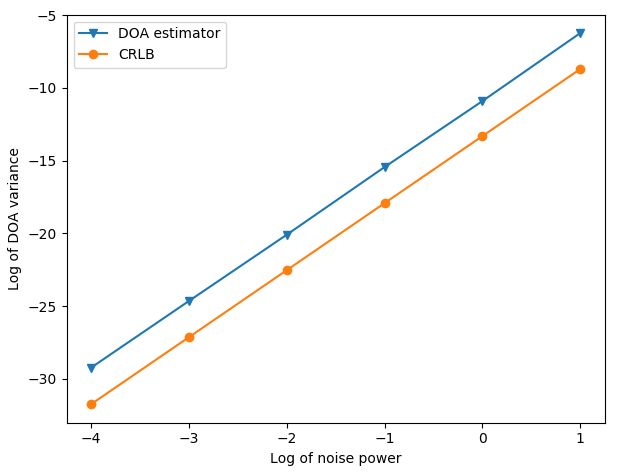
\includegraphics[scale=0.8]{CRLBcompare}
  \caption{Log-log plot of DOA estimator error vs. the Cramer Rao lower bound on FDOA-based DOA variance. }
  \label{CRLB}
\end{figure}

\begin{figure}
  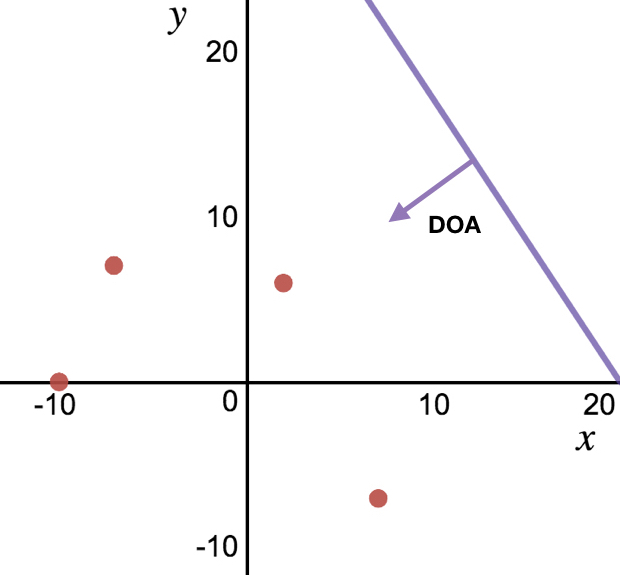
\includegraphics[scale=0.3]{sensor_config_arrow}
  \caption{Receiver configuration for CRB comparison in Fig.~\ref{CRLB}.}
  \label{config}
\end{figure}

Numerical trials can then be run with our DOA approximation method and the variance in DOA can be compared to the CRLB. This is the content of Figure \ref{CRLB}. The $x$-axis gives varying levels of noise power and the $y$-axis shows corresponding AOA variance for our approximation and the CRLB. It is clear that the AOA variance trend mimics that of the CRLB.
